%\documentclass[a4paper,11pt]{article}
\documentclass[a4paper,11pt]{scrartcl}

\usepackage[utf8]{inputenc}
\usepackage[italian]{babel}

\usepackage{graphicx} %for includng images
\graphicspath{{img/}}

\usepackage{siunitx} % package for deciBel and other units

\usepackage{amsmath} % package for ``cases'' and other matemagical stuff

\usepackage[american]{circuitikz} % circuit drawer
\ctikzset{/tikz/circuitikz/bipoles/length=1cm} %dimensione componenti

\usepackage{subcaption}  %per immagini multiple

%\usepackage{xcolor} % Colori!
\usepackage{colortbl} %colori nelle tabelle!!

\usepackage{multirow} %righe doppie nelle tabelle

\usepackage{makecell} %multirow box
\usepackage{hyperref}
\hypersetup{ % vedi https://it.overleaf.com/learn/latex/hyperlinks
    colorlinks=true,
    linkcolor=blue,
    filecolor=magenta,      
    urlcolor=blue
}
\title{Appunti di Principi di Ingegneria Elettrica II}
\author{Daniele Olivieri}
\date{}

\pdfinfo{%
  /Title    ()
  /Author   ()
  /Creator  ()
  /Producer ()
  /Subject  ()
  /Keywords ()
}
\includeonly{05_18_03_circuiti_laplace}
\begin{document}
\maketitle
Ti piacciono i miei appunti? Saranno sempre liberi e gratuiti ma puoi sostenermi con una donazione cliccando \href{https://www.paypal.com/donate?hosted_button_id=7KELP768NJSYW}{QUI}

Puoi accedere ai codici sorgente seguendo questo \href{https://github.com/FlashNoob98/appunti_principi_II_unina}{link} invece.
\setlength\arrayrulewidth{1.2pt} %larghezza righe tabelle
\section{Introduzione ai circuiti dinamici}
Tutti i circuiti che contengono componenti come
resistori, induttori e condensatori, generatori indipendenti di tensione e corrente ai quali si associa 
una tensione impressa o una corrente impressa vengono detti circuiti lineari tempo invarianti (LTI).

Se vi sono anche bipoli tempo-varianti come interruttori che si chiudono o si aprono, il circuito
si definisce lineare tempo variante (LTV).

Preso un generico circuito, si vuole determinare una tensione o un'intensità di corrente di un generico
bipolo.

\textbf{Strumenti a disposizione:}

\begin{itemize}
\item Equazioni di interconnessione:
\begin{equation} \label{eq:leggi_kirchooff}
\begin{cases}
        \text{LKC} & \forall \text{ nodo } \sum_{k} (\pm) i_k(t) = 0\ \forall\ t \\
        \text{LKT} & \forall \text{ maglia } \sum_{h} (\pm) v_n(t) = 0\ \forall\ t
\end{cases}
\end{equation}

\item Relazioni caratteristiche dei bipoli coerenti con la scelta dei versi delle grandezze (convenzione del generatore o dell'utilizzatore).
\begin{equation}
\begin{cases}
v_R  = R\cdot i \\
v_L  = L\frac{di_L}{dt} \\
i_C  = C\frac{dv_C}{dt} \\
v_e  = e(t)\\
i_j  = j(t) \\
\end{cases}
\end{equation}
\begin{equation*}
\begin{cases}
\text{interruttori in chiusura a t=0: }  {t<0,\ i = 0\ \forall\ v;\ t > 0,\ v = 0\ \forall\ i} \\
\text{interruttori in apertura a t=0: }  {t<0,\ v = 0\ \forall\ i;\ t > 0,\ i = 0\ \forall\ v} 
\end{cases}
\end{equation*}
\end{itemize}

Le equazioni di interconnessione non sono tutte indipendenti ma è sempre possibile
costruire un set di equazioni indipendenti scegliendo \textit{n-1} nodi o \textit{n-l-1} maglie fondamentali,
dove n ed l sono rispettivamente il numero di nodi e lati del grafo connesso.

NOTA: per ogni induttore la potenza assorbita:
$$ P^a(t) = v_l\cdot i_l = L \frac{di_L}{dt}\cdot i_l = \frac{d}{dt} \left[\frac{1}{2}Li_L^2\right] = \frac{dW_m}{dt} $$ 
L' energia immagazzinata nel campo magnetico dell'induttore invece:
$$\Delta W^a(t_1,t_2) = \int_{t_1}^{t_2} P^a(\tau)d\tau = W_m (t_2) - W_m(t_1) $$
Se in un certo istante di tempo l'induttore presenta una certa quantità di energia in Joule [\si{\joule}] quella sarà la massima energia estraibile.

Per ogni condensatore invece potenza ed energia sono così definite:
$$P^a(t) = \frac{d}{dt} W_e;\ W_e(t) = \frac{1}{2} CV_c^2$$
L'energia sarà immagazzinata mediante il campo elettrico.

Si ha quindi un sistema di equazioni circuitali in cui si ha una parte algebrica con le caratteristiche adinamiche, ossia con caratteristiche
non differenziali e non integrali, più una parte differenziale data dai bipoli dinamici come condensatori e induttori.
In letteratura un sistema simile si indica con DAE (Differential Algebric Equation), differente
dalla ODE (Ordinary Differential Equation).

Le tecniche utilizzate in teoria dei circuiti mirano a trasformare una DAE in una ODE, ossia 
formulare le equazioni circuitali come equazioni differenziali ordinarie, per operare questa trasformazione si fa 
riferimento alla dinamica delle sole {variabili di stato}: $i_l(t),\ v_c(t)$

La loro conoscenza permette di esprimere tutte le altre variabili attraverso relazioni algebriche, vengono definite
variabili \textit{slaved}, perché subordinate alle prime.

Per eseguire ciò si richiama una procedura generale per l'analisi di circuiti lineari tempo varianti (LTV).
Questa procedura si basa su un'analisi a intervallo: si partiziona l'asse dei tempi in intervalli in ciascuno dei 
quali esiste un circuito tempo invariante (LTI) equivalente a quello di partenza.

\begin{figure}[H] %tre stati diversi dello stesso circuito
\centering
 \begin{subfigure}{.3\textwidth}
  \centering
  \caption{configurazione generica}
  \begin{circuitikz}
   \draw (0,0) to [R] (1,0);
   \draw (0,0.6) to [L] (1,0.6);
   \draw (0,1.2) to [C] (1,1.2);
   \draw (0,1.8) to [V] (1,1.8);
   \draw (0,2.4) to [I] (1,2.4);
   \draw (0,3) to [closing switch] (1,3);
   \draw (0,3.6) to [opening switch] (1,3.6);
   \draw (-0.3,-0.3) rectangle (1.3,3.9);
  \end{circuitikz}
 \end{subfigure}
 \begin{subfigure}{.3\textwidth}
  \centering
  \caption{$t<0$}
  \begin{circuitikz}
   \draw (0,0) to [R] (1,0);
   \draw (0,0.6) to [L] (1,0.6);
   \draw (0,1.2) to [C] (1,1.2);
   \draw (0,1.8) to [V] (1,1.8);
   \draw (0,2.4) to [I] (1,2.4);
   \draw (0,3) to [open,o-o] (1,3);
   \draw (0,3.6) to [short] (1,3.6);
   \draw (-0.3,-0.3) rectangle (1.3,3.9);
  \end{circuitikz}
 \end{subfigure}
 \begin{subfigure}{.3\textwidth}
  \centering
  \caption{$t>0$}
  \begin{circuitikz}
   \draw (0,0) to [R] (1,0);
   \draw (0,0.6) to [L] (1,0.6);
   \draw (0,1.2) to [C] (1,1.2);
   \draw (0,1.8) to [V] (1,1.8);
   \draw (0,2.4) to [I] (1,2.4);
   \draw (0,3) to [short] (1,3);
   \draw (0,3.6) to [open,o-o] (1,3.6);
   \draw (-0.3,-0.3) rectangle (1.3,3.9);   
  \end{circuitikz}
 \end{subfigure}
\end{figure}

Supponendo che i generatori indipendenti abbiano grandezze \textbf{limitate}, ossia le tensioni impresse $e(t)$ e le correnti impresse $j(t)$,
in questa ipotesi si sa che le variabili di stato sono funzioni \textbf{continue} ossia:
\begin{equation*}
\begin{split}
i_L (0^+) & = i_L(0^-) \\
v_C (0^+) & = v_C(0^-)
\end{split}
\end{equation*}

La soluzione si determina trovando la dinamica delle variabili di stato in ciascun circuito ausiliario, "incollando" le soluzioni utilizzando la proprietà di continuità delle variabili di stato.

Il problema di risolvere circuiti lineari tempo varianti si scompone nel risolvere tanti circuiti lineari tempo invarianti. Una categoria semplice di circuiti tempo invarianti sono i
circuiti lineari del primo ordine (circuiti RC o RL) con un solo elemento dinamico.
\begin{figure}[H] %circuiti RC ed RL equivalenti
\centering
 \begin{subfigure}{.3\textwidth}
  \centering
  \begin{circuitikz}
   \draw (0,0) rectangle (1.6,1.7);
   \draw (0.3,0.3) to [I] (1.3,0.3);
   \draw (0.3,0.9) to [V] (1.3,0.9);
   \draw (0.3,1.5) to [R] (1.3,1.5);
   \draw (1.6,1.5) to [short,i=$i_C$] (2,1.5)
   to [C,v^=$v_C $] (2,0.4) to [short] (1.6,0.4);
  \end{circuitikz}
  \caption{Circuito RC}
 \end{subfigure} 
  \begin{subfigure}{.3\textwidth}
  \centering
  \begin{circuitikz}
   \draw (0,0) rectangle (1.6,1.7);
   \draw (0.3,0.3) to [I] (1.3,0.3);
   \draw (0.3,0.9) to [V] (1.3,0.9);
   \draw (0.3,1.5) to [R] (1.3,1.5);
   \draw (1.6,1.5) to [short,i=$i_L $] (2,1.5)
   to [L,v^=$v_L $] (2,0.4) to [short] (1.6,0.4);
  \end{circuitikz}
  \caption{circuito RL}
 \end{subfigure}
\end{figure}

Un bipolo adinamico lineare e un bipolo dinamico fanno subito pensare all'utilizzo dei teoremi di Thévenin e Norton, permettendo la riduzione del circuito 
adinamico ad un semplice generatore con un resistore equivalente.

Applicando ad esempio la LKT $e_0(t) = R_{th}\cdot C \frac{dV_C}{dt} + V_C$ si ha l'equazione di stato
del circuito e supponendo di conoscere $V_C(t=0) = V_0 $ allora la soluzione dell'equazione è:
$$V_C(t) = [V_0-V_{C_p}(0)] e^{-\frac{t}{\tau}} + V_{C_p}(t)$$ dove $\tau = R_{th}\cdot C$ e $V_{C_p}(t)$
è la soluzione a regime. 
 
Dopo un intervallo pari a $4\sim 5\ \tau$ si assume il processo di carica o scarica terminato.

Per il circuito RL 
$$I_L(t) = [I_0-I_{L_p}(0)]e^{-\frac{t}{\tau}} + I_{L_p}(t)$$ 
con $\tau = \frac{L}{R_{th}},\ I_0 = I_L (t=0)$

Osservazione: la soluzione generale del circuito RC, ossia la dinamica di $V_c(t)$ può essere espressa 
come la somma di due termini $V_{C_{tr}}(t)$ e $V_{C_p}(t)$, il primo transitorio, che tende a svanire se 
si attende un tempo sufficiente lungo, porta con se la \textit{memoria} dello stato iniziale, memoria che 
viene
persa quando $t>4\sim5\ \tau$, ammesso che $\tau$ sia positiva; esistono infatti alcune combinazioni di 
elementi circuitali che si comportano come un resistore negativo.

Il secondo termine è quello di regime permanente, che ovviamente non ha memoria dello stato iniziale ma 
dipende solo dalla nuova configurazione
del circuito (termine forzato).

La decomposizione in regime transitorio e permanente è una decomposizione generale che vale per qualsiasi circuito, a patto di complicare opportunamente la matematica.

Si parla quindi di evoluzione libera ed evoluzione forzata 
$$\begin{cases}
e_0(t) = R_{th}C\frac{dV_c}{dt} + V_C \\
V_c(0) = V_0
\end{cases}$$
si scompone in:

Evoluzione libera
$$\begin{cases}
0 &= R_{th}C\frac{dV_c}{dt} + V_C \\ 
V_c(0) &= V_0
\end{cases}$$

Evoluzione forzata
$$\begin{cases}
e_0(t) &= R_{th}C\frac{dV_c}{dt} + V_C \\
V_c(0) &= 0
\end{cases}$$

Trattazione analoga (duale) per il circuito RL

\newpage
\subsection{Circuiti lineari tempo invarianti del II ordine}
Divisi in (RC, RL, RLC), la procedura generale di risoluzione richiede tre step:
\begin{enumerate}
 \item Determinazione delle equazioni di stato
 \item Determinazione delle condizioni iniziali
 \item Soluzione del problema di Cauchy
\end{enumerate}

Esempio:
\begin{figure}[H]
\centering
\begin{circuitikz}
 \draw (0,2) to [V,l_=$E$] (0,0);
 \draw (0,2) to [closing switch=${t=0}$](1,2) 
             to [R,l=$R_1$] (2.5,2)
             to [R,l=$R_2$] (4,2)
             to [L,i=$i_L$,l=$L$] (4,0)
             to [short] (0,0);
 \draw (2.5,2)node[circ,color=red]{} to [C,v=$v_C$,l=$C$] (2.5,0);
\end{circuitikz}
\caption{Esempio di un circuito RLC del secondo ordine}
\end{figure}

La dinamica dello stato per $t<0$ è di facile risoluzione, $i_L(t) = 0$, $v_C(t) = 0$
per $t > 0$ invece si analizza il circuito:

Equazioni di interconnessione: 
LKC nel nodo evidenziato in rosso (tra i due resistori)
\begin{equation*}
\begin{cases}
I_1 &= I_C+i_L \ \qquad \text{LKC}\\
E &= R_1\cdot I_1 + v_C\ \qquad \text{LKT} \\
v_C &= R_2 \cdot i_L + V_L\ \qquad \text{LKT} \\
V_L &= L\frac{di_L}{dt} \\
I_C &= C\frac{dv_C}{dt}
\end{cases}
\end{equation*}
Si ricava $I_1$ dalla seconda e si sostituisce nella prima,
ora si ricavano le variabili di stato ottenendo
$$
\begin{cases}
i_C = \frac{E}{R_2} - \frac{v_C}{R_1} - i_L \\
v_L = v_C - R_2 i_L
\end{cases}
$$
Sostituendo le equazioni caratteristiche dei bipoli dinamici:

$$
\begin{cases}
C\frac{dv_C}{dt} = \frac{E}{R_2} - \frac{v_C}{R_1} - i_L \\
L\frac{di_L}{dt} = v_C - R_2 i_L
\end{cases}
$$

Le condizioni iniziali sono 
$$\begin{cases}
v_C(0^+) = v_C(0^-) = 0\\
i_L(0^+) = i_L(0^-) = 0
\end{cases}
$$
Per risolvere queste equazioni conviene ridurle ad un'equazione del secondo ordine ad una sola incognita,
ad esempio si sostituisce nell'equazione che definisce $i_C$, $v_C$ ricavata dalla equazione di
$v_L$, in questo modo si ha un'unica equazione in cui compaiono le grandezze relative all'induttore.

Si ottiene 
\begin{equation}
LC \frac{d^2i_L}{dt^2} + CR_2\frac{di_L}{dt} = \frac{E}{R_1} - \frac{L}{R_1}\frac{di_L}{dt} - \frac{R_2}{R_1}i_L-i_L
\end{equation}
raccogliendo i termini
$$
\frac{d^2i_L}{dt^2} + \left(\frac{R_2}{L} + \frac{1}{R_1C}\right)\frac{di_L}{dt}+ \left(1 + \frac{R_2}{R_1}\right)\frac{1}{LC} i_L = \frac{E}{R_1}\frac{1}{LC}
$$
%ora raccogli i termini
Controlli da eseguire: controllo dimensionale e positività dei coefficienti altrimenti il circuito non sarebbe dissipativo.

L'integrale generale è scritto come somma dell'integrale dell'omogenea associata e dell'integrale particolare.
Si ottiene il polinomio caratteristico a partire dall'omogenea associata, ossia annullando il forzamento:
\begin{equation}
\lambda^2 + \left(\frac{R_2}{L} + \frac{1}{R_1 C}\right)\lambda + \left(1+\frac{R_2}{R_1}\right)\frac{1}{LC} = 0
\end{equation}
La soluzione del polinomio può essere di tre tipi:

\begin{itemize}
\item Caso 1, radici reali e distinte, solitamente negative in sistemi dissipativi, modi naturali aperiodici 
smorzati
$$
i_{L_0} = K_1 e^{\lambda_1 t} + K_2 e^{\lambda_2 t}
$$
\begin{figure}[H]
\centering
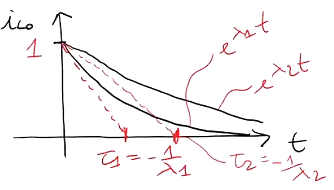
\includegraphics[width=0.4\linewidth]{evoluzione_libera_reali_distinte}
\end{figure}


\item Caso 2, radici reali e coincidenti, caso piuttosto patologico
la radice viene determinata con $-\sigma$ si avrà un modo esponenziale decrescente $e^{-\sigma t} $ con
$\tau = \frac{1}{\sigma}$ e un modo pari a  $t\cdot e^{-\sigma t}$
$$
i_{L_0} = K_1 e^{-\sigma t} + K_2 t\cdot e^{-\sigma t}
$$
\begin{figure}[H]
\centering
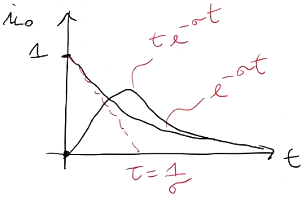
\includegraphics[width = 0.4\linewidth]{evoluzione_libera_reali_coincidenti}
\end{figure}
Vengono detti modi aperiodici smorzati con smorzamento critico.


\item Caso 3, modi periodici smorzati, soluzioni complesse coniugate
$\lambda_{1,2} = -\sigma \pm j\omega_d$, la distanza tra due picchi è pari a $\frac{2\pi}{\omega_d}$
$$i_{L_0}(t) = e^{-\sigma t} [K_1 \cos (\omega_d t) + K_2 \sin(\omega_d t)]$$
\begin{figure}[H]
\centering
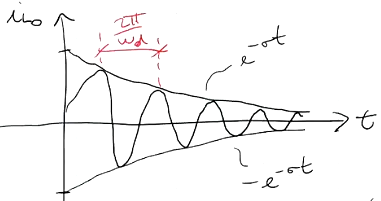
\includegraphics[width=0.4\linewidth]{evoluzione_libera_complesse_coniugate}
\end{figure}
\end{itemize}

Restano da determinare le costanti di integrazione imponendo le condizioni iniziali,
\begin{equation*}
\begin{cases}
i_L(0^+) = i_L(0^-) = \SI{0}{\ampere}\\
\frac{di_L}{dt}(0^+) = \frac{1}{L}[v_C(0^+) - R_2i_L(0^+)] = 0
\end{cases}
\end{equation*}

Supponendo dunque di avere soluzioni $\lambda_1,\ \lambda_2$ reali e distinte e ricordando di aggiungere
il termine a regime $\frac{E}{R_1 + R_2}$ nella determinazione dei coefficienti
$$
\begin{aligned}
i_L(0^+) = 0 & \Rightarrow \\
\frac{di_L}{dt}(0^+) = 0 & \Rightarrow
\end{aligned}
\begin{cases}
K_1+K_2 + \frac{E}{R_1+R_2} = 0 \\
\lambda_1K_1 + \lambda_2K_2 = 0
\end{cases}
$$
La soluzione del sistema permette di ricavare i coefficienti $K_1$ e $K_2$

%Lezione 2 i minuti si riferiranno a quelli visibili su teams e non quelli del file registrato con OBS
\section{Determinazione equazioni di stato di un circuito qualsiasi}

Si riprende la classe di circuiti lineari tempo invarianti (LTI), supponiamo di conoscere
le variabili di stato $i_L(t) $ e $v_C(t) $ assumendole note, sostituiamo ogni \textit{condensatore}
con un generatore di tensione di valore pari alla $v_C(t)$ , ripetendo il procedimento
per ciascun \textit{induttore} che viene sostituito con un generatore di corrente con corrente impressa
pari a $i_L(t)$.

In queste condizioni, la soluzione del circuito resta formalmente invariata.
Il nuovo circuito sarà di tipo adinamico, non presenterà più alcun componente dinamico, il nuovo circuito
prende il nome di \textit{circuito resistivo associato al circuito di partenza}.

Il vantaggio di questa operazione è la possibilità di ricavare $v_L$ e $i_C$ utilizzando il principio
di \textit{sovrapposizione degli effetti} (PSE).

Si ricavano le equazioni di stato per il seguente circuito:
26:07

\begin{figure}[h]

\end{figure}

Si applica il PSE, per trovare $i_C$ e $v_L$:
$$
i_C = i_c' + i_C'' + i_C '''
$$
$$
v_L = v_L' + v_L'' + v_L'''
$$

Disegna circuiti 28:48

Circuito 1)
$$
v_L' = 0;\ i_C' = \frac{E}{R_1} 
$$
Circuito 2)
$$
i_C'' = -\frac{v_C}{R_1};\ v_L'' = v_C
$$
Circuito 3)
$$
i_C''' = -i_L;\ v_L''' = -R_2\cdot i_L
$$

Sommando i tre contributi:
$$
i_C = \frac{E}{R_1} - \frac{v_C}{R_1} - i_L = C\frac{dv_C}{dt}
$$
$$
v_L = v_C - R_2\cdot i_L = L\frac{di_L}{dt}
$$
con le condizioni di continuità delle variabili di stato:
$$
i_L(0^+) = i_L(0^-)
$$
$$
v_C(0^+) = v_C(0^-)
$$

\section{Circuiti lineari con generazioni impulsivi}
Si analizza ora un circuito che presenta generatori di tipo impulsivo, ad esempio la risposta di 
una linea elettrica a seguito di una fulminazione.
Si definisce quindi l'impulso rettangolare di ammpiezza $\Delta$, la funzione viene chiamata 
$\Pi_\Delta(t)$,(funzione porta) è costante nell'intervallo $[-\frac{\Delta}{2},\frac{\Delta}{2}]$,
l'area del rettangoloide sotteso alla funzione è pari a
$$
\int_{-\Delta/2}^{\Delta/2}\Pi_\Delta(\tau)d\tau = 1\ \forall\ \Delta \in\ ]0,+\infty[
$$
Ha senso considerare la successione di funzioni ottenute per valori $\Delta$ decrescenti,
ma dimezzando la base, per mantenere l'area unitaria, va raddoppiata l'altezza.

Passando al limite per $\Delta \rightarrow 0^+$ la successione tende in maniera non ordinaria
ad un limite che non è una funzione ma può essere definita come funzione generalizzata,
ossia distribuzione, che prende il nome di \textbf{Delta di Dirac} ($\delta(t)$).

Proprietà della delta:
\begin{itemize}
\item È nulla $\forall t \neq 0$
\item Ha integrale unitario
\item Proprietà di campionamento $\int_{-\infty}^{+\infty}f(\tau)\delta(\tau-t_0)d\tau = f(t_0)$
\end{itemize}
Esempio della proprietà di campionamento: 49:03
$$
\int_{-\Delta/2}^{\Delta/2} f(\tau)\Pi_\delta(\tau-t_0)d\tau = \frac{1}{\Delta} \int_{-\Delta/2}^{\Delta/2}  f(\tau)d\tau = f(\vartheta^*)
$$


Analizziamo un'altra funzione $U_\Delta(t)$ definita come segue:
\begin{equation*}
\begin{cases}
0\ ,& t  < -\frac{\Delta}{2} \\
1\ ,& t  > \frac{\Delta}{2} \\
\frac{1}{2}+\frac{t}{\Delta}\ ,& -\frac{\Delta}{2} \leq t \leq \frac{\delta}{2}
\end{cases}
\end{equation*}
Rampa 55:03

Eseguendo la derivata temporale si otterrà la funzione $\Pi_\Delta(t)$, al limite di $\Delta \rightarrow 0$
si ottiene la funzione definita ``gradino'' o funzione di Heaviside $u(t)$.

Un ulteriore modo per definire la $\delta(t)$ è appunto quella di derivata della funzione gradino $u(t)$.
$$
\delta(t) = \frac{d}{dt}u(t) \Leftrightarrow \int_{-\infty}^t \delta(\tau)d\tau = u(t)
$$

\paragraph{Esempio con generatore impulsivo}
Si prenda un circuito RC serie 01:12:00 e una funzione $e(t)$ che vale $E_0$ per $0 < t < T$ e $0$ 
altrimenti.
Ricaviamo $v_C(t)$:

Si suppone che la condizione iniziale, ossia per $t < 0 $, la tensione sul condensatore sia nulla.

\begin{equation*}
\begin{cases}
e(t) &= RC\frac{dv_C}{dt} + v_C \\
v_C(0) &= 0
\end{cases}
\end{equation*}

$$
\begin{cases}
E_0 &= RC\frac{dv_C}{dt} + v_C \\
v_C^{(1)}(0) &= 0 \\
0 \leq t \leq T
\end{cases}
$$

$$
\begin{cases}
0 &= RC\frac{dv_C}{dt} + v_C \\
v_C^{(2)}(0) &= v_C^{(1)}(T) \\
t \geq T
\end{cases}
$$
Rivedi 1:19:00

Si ottiene una funzione esponenziale crescente fino a $T$ e poi decrescente fino a 0 all'infinito.
Diminuendo il valore di $T$ si vede che il ``picco'' della funzione sarà più basso, al limite 
di $T \rightarrow 0$ la soluzione si annulla.
Se imponiamo il prodotto $E_0\cdot T = 1$ ed eseguiamo il limite invece:
$$
\lim_{T\rightarrow0^+} v_C(t)
$$
Supponiamo di sviluppare la funzione esponenziale con la sua serie di Taylor:
$$
e^x = 1 + x + \frac{x^2}{2!} + \frac{x^3}{3!} + ... \Rightarrow 1-e^{-\frac{t}{\tau}} \simeq \frac{t}{\tau} 
$$

$$
\begin{cases}
0\ & t\leq 0 \\
\frac{1}{T}\frac{t}{\tau}\  & 0 \leq t\leq T \\
\frac{1}{T}\frac{T}{\tau} e^{-\frac{t-T}{\tau}}\ & t\geq T
\end{cases}
$$
Per $T\rightarrow 0^+$
$$
\begin{cases}
0\ & t\leq 0\\
\frac{1}{\tau}e^{\frac{-t}{\tau}}\ & t \geq 0
\end{cases}
$$

Il primo tratto dell'equazione si approssima quindi ad un tratto lineare fino a T, arrivando ad 
un'altezza di $\frac{1}{\tau}$ vedi figura 1:32:00

Se 
$$\Pi_\Delta(t) \stackrel{\Delta\rightarrow0^+}{\rightarrow} \delta(t) \Rightarrow v_C(t) \rightarrow h(t)$$
$h(t)$ è chiamata risposta all'impulso del circuito dinamico.

$$
\delta(t) = RC\frac{dv_C}{dt} + v_C \Leftarrow i_C = \frac{\delta(t)-v_C}{R}
$$
Se la tensione è impulsiva anche la corrente nel condensatore sarà di tipo impulsivo
$$
i_c = C\frac{dv_C}{dt} \Rightarrow \int_{0^-}^{0^+} i_C(\tau)d\tau = e[v_C(0^+)-v_C(0^-)]
$$
$$
v_C(0^+) - v_C(0^-) = \frac{1}{RC} \int_{0^-}^{0^+} \delta(\tau)d\tau - \frac{1}{RC} \int_{0^-}^{0^+} v_C(\tau)d\tau = \frac{1}{RC} = \frac{1}{\tau} \Rightarrow 
$$
$$
\Rightarrow v_C(0^+) = \frac{1}{RC} = \frac{1}{\tau}
$$
Rivedi discorso potenza 1:44:00

\paragraph{Risposta al gradino unitario di un circuito dinamico LTI}
Stesso circuito del precedente, ma stavolta si utilizza come forzamento il gradino unitario di
Heaviside, la soluzione è più semplice della precedente:

$$
v_C(t) = 1-e^{-\frac{t}{\tau}}u(t)
$$
la chiamiamo $g(t)$ e affermiamo che sia la risposta al gradino, richiamiamo la relazione
tra la funzione $\Pi_\Delta(t)$ e $U_\Delta(t)$ si ha che:
$$
\Pi_\Delta(t) = \frac{U_\Delta\left(t+\frac{\Delta}{2}\right)-U_\Delta\left(t-\frac{\Delta}{2}\right)}{\Delta} = e(t)
$$
per $\Delta \rightarrow 0^+$ ottengo $h(t) = v_C(t)$.

Essendo il circuito tempo invariante, si può trovare la risposta alla funzione $\Pi_\Delta(t)$
come combinazione lineare delle risposte delle due $U_\Delta$ opportunamente traslate, ossia
la risposta al gradino traslata.
$$
\text{Risp} \Pi_\Delta(t) = \frac{\text{Risp}\left\{U_\Delta\left(t+\frac{\Delta}{2}\right)\right\} - 
\text{Risp}\left\{U_\Delta\left(t-\frac{\Delta}{2}\right)\right\}}{\Delta} = 
\frac{g\left(t+\frac{\Delta}{2}\right) - g\left(t-\frac{\Delta}{2}\right)}{\Delta}
$$
Tutto si trasforma nella funzione rapporto incrementale della funzione $g(t)$ ossia
$$
\lim_{\Delta\rightarrow0^+}\text{Risp}\left\{\Pi_\Delta(t)\right\} = h(t) = \frac{dg}{dt}
$$

$$
h(t) = \frac{dg}{dt} = 0,\ t < 0;\ \frac{1}{\tau}e^{-\frac{t}{\tau}},\ t\geq0 
$$
La risposta all'impulso è quindi la derivata della risposta al gradino.

Si consideri un circuito RC serie
\begin{figure}[H]\centering
\begin{circuitikz}
\draw
(0,0) to [voltage source,invert,l=$u(t)$] (0,2)
      to [R=$R$] (2,2)
      to [C,l_=$C$,v^=$v_C$] (2,0) -- (0,0)
;
\end{circuitikz}
\end{figure}
si suppone che la tensione imposta al generatore sia un gradino unitario $u(t)$,
l'equazione di stato sarà:
$$
\begin{cases}
u(t) = RC \frac{dv_C}{dt} + v_C \\
v_C(0^+) = 0
\end{cases}
\Rightarrow v_C(t) = \left.
\begin{cases}
0 & t<0 \\
1-e^{-\frac{t}{\tau}} & t\geq 0
\end{cases}\right] = g(t)
$$

Si considera la funzione $U_\Delta$
$$U_\Delta(t) = 
\begin{cases}
0 & t< -\frac{\Delta}{2}\\
\frac{1}{2} + \frac{t}{\Delta} & -\frac{\Delta}{2} < t < \frac{\Delta}{2} \\
1 & t > \frac{\Delta}{2}
\end{cases}
$$
se si esegue la differenza di due funzioni $U_\Delta$ traslate di $\pm\frac{\Delta}{2}$ si ottiene 
una porta trapezoidale
$$
f(t) = \frac{U_\Delta\left(t+\frac{\Delta}{2}\right) - U_\Delta\left(t-\frac{\Delta}{2}\right)}{\Delta}
$$
tende ad una $\delta(t)$ delta di Dirac per $\Delta \rightarrow 0$.
Semplicemente si può invece definire la porta come differenza di due gradini traslati, in questo modo
si elimina il problema dei segmenti obliqui.

La linearità del sistema e la tempo-invarianza delle grandezze dei bipoli implica che la
risposta ad una combinazione lineare di funzioni traslate nel tempo si ottiene come combinazione lineare 
delle risposte dei singoli termini traslati.
$$
\text{Risp}\left\{\Pi_\Delta(t)\right\} = \frac{\text{Risp}\left\{u\left(t+\frac{\Delta}{2}\right) \right\} -\text{Risp}\left\{ u\left(t-\frac{\Delta}{2}\right) \right\}}{\Delta} = \frac{g\left(t+\frac{\Delta}{2}\right)-
g\left(t-\frac{\Delta}{2}\right)}{\Delta}
$$
Eseguendo il limite per $\Delta\to 0^+ $ si vede che quello appena presentato è un rapporto incrementale e
quindi
$$
\lim_{\Delta\to0^+} \Rightarrow \text{Risp} \left\{\delta(t)\right\} =h(t) = \frac{dg}{dt}
$$
Ricordando le funzioni $h(t)$ e $g(t)$ si vede la relazione
$$
h(t) = \begin{cases}
0 & t<0\\
\frac{1}{\tau}e^{-\frac{t}{\tau}} & t\geq 0
\end{cases}\qquad
g(t) = \begin{cases}
0 & t<0\\
1 - e^{-\frac{t}{\tau}} & t\geq 0
\end{cases} \Rightarrow
\frac{dg}{dt} = h(t)
$$
è possibile studiare la risposta all'impulso sfruttando quella al gradino, che è una funzione limitata e 
più semplice da analizzare.

\paragraph{Circuiti RC ed RL semplici con generatori impulsivi}
Si considerino 2 circuiti modello: il circuito RC parallelo e il circuito RL serie.

\begin{figure}[H]\centering
\begin{subfigure}{.4\textwidth}\centering
\begin{circuitikz}
\draw
(0,0) to [current source,l=$j(t)$] (0,2)
      to (1,2) to [R=$R$,i>^=$i_R$] (1,0) to (0,0);
\draw
(1,2) to (2.5,2)  to [C,l_=$C$,v^=$v_C(t)$,i>_=$i_C$] (2.5,0) -- (1,0)
;
\end{circuitikz}
\subcaption{RC parallelo}
\end{subfigure}
\begin{subfigure}{.4\textwidth}\centering
\begin{circuitikz}
\draw
(0,0) to [voltage source,invert,l=$e(t)$] (0,2)
      to [R,l_=$R$] (2.5,2) to [L,l_=$L$,i_>=$i_L(t)$,v^=$v_L$] (2.5,0) -- (0,0)
;
\end{circuitikz}
\subcaption{RL serie}
\end{subfigure}
\end{figure}

Siano i generatori impulsivi: $j(t) = Q\delta(t)$ ed $e(t) = \Phi\delta(t)$.
$$
j(t) = \frac{v_C}{R} + i_C = Q\delta(t) = \frac{v_C}{R} + C\frac{dv_C}{dt}
$$
Si integra la funzione nell'istante in cui è centrata la $\delta(t)$ ossia:
$$
\int_{0^-}^{0^+} Q\delta(\tau)d\tau  = \cancel{\int_{0^-}^{0^+}\frac{v_C}{R}d\tau} + C[v_C(0^+)-\cancel{v_C(0^-)}]
\Leftrightarrow Q = Cv_C(0^+) \ \ [Q] = \si{\coulomb} \text{ (Coulomb)}
$$
$$
\left[\int_{0^-}^{0^+} Q\delta(\tau)d\tau\right] = \text{ Coulomb}
$$
Tirando la costante $C$ fuori dall'integrale, che ha la dimensione di Coulomb, l'integrale rimanente
deve essere adimensionale.
Ciò significa che la $\delta(t)$ ha la dimensione di \si{\per\second} per essere coerente con l'integrale
e restituire una quantità finita.

\subparagraph{Caso duale con circuito RL:}

$$
e(t) = R\cdot i_L + v_L
$$
$$
\Phi\delta(t) = R\cdot i_L + L\frac{di_L}{dt}
$$
$$
\Phi\int_{0^-}^{0^+} \delta(\tau)d\tau = L i_L(0^+)\ , \ i_L(0^-) = 0
$$

Anche in questo caso per avere la dimensione del flusso in \si{\weber} per $\Phi$ allora la $\delta(t)$ 
avrà le dimensioni di \si{\per\second}.
\newpage
\subsection{Procedura generale per la risoluzione di circuiti con generatori impulsivi}
Si ha un circuito dinamico semplice al quale è collegato un generatore impulsivo,
si determina il circuito resistivo associato, ossia vengono sostituiti i condensatori con 
generatori di tensione e gli induttori con generatori di corrente.

Si ottiene un circuito parziale in cui si spengono i generatori interni (anche quelli equivalenti ai bipoli dinamici) e si lascia agire solo il generatore impulsivo.

Un ulteriore circuito è ottenuto facendo l'esatto contrario e spegnendo quindi il generatore impulsivo.

\begin{figure}[H]\centering
\begin{subfigure}{0.45\linewidth}\centering
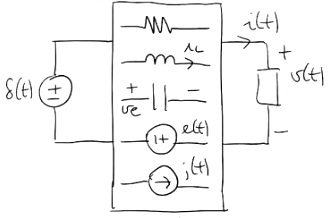
\includegraphics[width=\linewidth]{lezione_03_circuito_A}
\subcaption{Circuito iniziale}
\end{subfigure}
\begin{subfigure}{0.45\linewidth}\centering
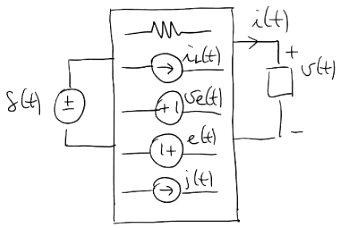
\includegraphics[width=\linewidth]{lezione_03_circuito_B}
\subcaption{Circuito resistivo associato}
\end{subfigure}
\begin{subfigure}{0.45\linewidth}\centering
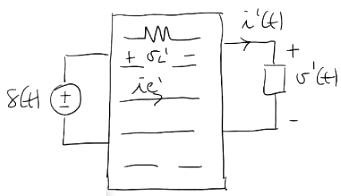
\includegraphics[width=\linewidth]{lezione_03_circuito_C-}
\subcaption{Circuito C'}
\end{subfigure}
\begin{subfigure}{0.4\linewidth}\centering
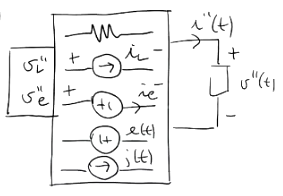
\includegraphics[width=\linewidth]{lezione_03_circuito_C--}
\subcaption{Circuito C"}
\end{subfigure}
\end{figure}
37:19
Si applica il PSE (Principio di Sovrapposizione degli effetti)
$$
\begin{cases}
v_L = v_L' + v_L''\\
i_C = i_C' + i_C''
\end{cases}
$$

Dal circuito C' si ricavano $v_L'$ e $i_C'$ causate dai generatori impulsivi 41:41

Viceversa dal circuito C'' si valutano le variabili di stato utilizzando come condizioni iniziali
le variabili ottenute in C'.

$$
v_C(0^+) = \frac{1}{C} \int_{0^-}^{0^+} i_C'(\tau)d\tau \ , \ v_C(0^-) = 0
$$
$$
i_L(0^+) = \frac{1}{L} \int_{0^-}^{0^+} i_L'(\tau)d\tau \ , \ i_L(0^-) = 0
$$
L'integrale delle variabili di stato del circuito C'' è pari a 0 dato che la funzione integranda è limitata
e l'intervallo è infinitesimo.

Infine si risolve il circuito C'' usando le variabili di stato appena calcolate in C'.

Esercizio 

Conclusione dell'esercizio: le variabili di stato possono essere discontinue ma limitate, le altre
variabili possono invece essere anche impulsive.

\paragraph{Risposta forzata di un circuito LTI}
Si suppone di avere un solo generatore esterno, se ne vogliono determinare le variabili ai capi
di un solo bipolo, si parla di filtro o sistema SISO \textit{(Single Input Single Output)},
sia $x(t)$ l'ingresso e $y(t)$ l'uscita, si deve supporre che il circuito sia a stato 0, ossia
le sue variabili di stato sono tutte nulle (circuito precedentemente spento).

Si parla di approssimazione \textit{PieceWise-Constant} ossia costante a tratti dell'ingresso
$x(t)$.
Si partiziona l'asse dei tempi in tanti intervalli di ampiezza $\Delta t$ centrati negli istanti
di tempo $t_k = k\Delta t\ ,\ k\ \in\ Z$.

Costruiamo un'approssimazione $x_\Delta(t)$ costante di valore $x(t_k)$ in $\left[t_k-\frac{\Delta t}{2}\ ,\ 
t_k+\frac{\Delta t}{2}\right]$.
La funzione $x(t)$ può quindi essere rappresentata come somma di impulsi rettangolari successivi,
sfruttando la funzione $\Pi_{\Delta}(t)$, sarà quindi:
$$
x_{\Delta}(t) = \sum_{k = -\infty}^{+\infty} x(t_k) \Pi_\Delta(t-t_k)\Delta t
$$
Eseguendo il limite per $\Delta t \rightarrow 0^+$ in ipotesi di sufficiente regolarità:
$$
\lim_{\Delta t \to 0^+} x_\Delta(t) = x(t) = \int_{-\infty}^{+\infty} x(\tau) \delta (t-\tau)
d\tau
$$
Questa conclusione richiama la proprietà di campionamento della $\delta(t)$.

Se vogliamo calcolare la risposta di $x(t)$ allora:
$$
\text{Risp}\left\{x(t)\right\} = y(t) = \text{Risp} \left\{\int_{-\infty}^{+\infty} x(\tau)\delta(t-\tau)
d\tau\right\}
$$
per linearità e tempo-invarianza si ottiene
$$
y(t) = \int_{-\infty}^{+\infty} x(\tau)h(t-\tau) d\tau
$$
chiamato integrale di convoluzione, $h(t)$ è la risposta impulsiva per la variabile di uscita.

Si parla di prodotto di convoluzione tra due funzioni $f,g \ \in\ R$
$$
f * g(t) = \int_{-\infty}^{+\infty} f(\tau)g(t-\tau)d\tau
$$
Si può calcolare la risposta impulsiva... rivedi 1:57:00


Data la risposta all'ingresso impulsivo, si può calcolare la risposta a qualsiasi ingresso, mediante
l'uso dell'integrale di convoluzione.
Osservando attentamente l'integrale si vede che la risposta impulsiva gode della proprietà per la quale
$$
h(t) = 0 \ t<0,\ h(t) \neq 0 \forall t\ \geq 0 \Rightarrow t - \tau \geq 0 \Rightarrow \tau \leq t
$$

Se l'ingresso $x(t) = 0,\ t< t_0$ allora possiamo affermare che la $y(t)$ avrà come estremi di integrazione
$t_0^-$ e $t$, con il - si sottintende la possibilità che siano presenti $\delta(t_0)$ in quell'istante 
di tempo.

\paragraph{Esempi dell'utilizzo dell'integrale di convoluzione}
Circuito RC parallelo con forzamento esponenziale, forzato da un generatore di corrente.
$$
j(t) = I e ^{\frac{t}{\tau}} u(t)
$$
Per studiare la risposta del circuito bisogna per prima cosa determinare la $V_{cf}(t)$, mediante
lo studio della risposta impulsiva.
Per determinare la risposta impulsiva si forza il circuito con una $\delta(t)$, utilizzando i metodi 
precedenti.

$i_c = \delta(t)$
$$
v_c(0^+) = \frac{1}{C}\int_{0^-}^{0^+} i_c(\tau)d\tau + V_c(0^-) = \frac{1}{C}
$$
Per determinare la risposta impulsiva si determina l'evoluzione libera spegnendo il generatore,
ci sarà un parallelo RC con la seguente equazione di stato:
$$
\begin{cases}
RC\frac{dV_c}{dt} + v_C = 0 \\
V_c(0^+) = \frac{1}{C}
\end{cases}
$$
Quindi 
$$
V_{c_{lib}} = h(t) = \frac{1}{C} e^{-\frac{t}{RC}},\ t\geq 0
$$
$$
h(t) = \frac{1}{C}e^{-\frac{t}{RC}}\cdot u(t) \forall t
$$

Utilizzando l'integrale di convoluzione per calcolare la risposta forzata:

$$
V_{cf}(t) = \int_{0^-}^{t}Ie^{\frac{\tau}{T}} \cdot \frac{1}{C} e^{-\frac{t-\tau}{RC}} d\tau = 
\frac{I}{C} \int_{0^-}^{t} e^{\frac{\tau}{t}}\cdot e^{-\frac{t}{RC}}\cdot e^{\frac{\tau}{RC}} d\tau
$$

$$
= \frac{I}{C} e^{-\frac{t}{RC}}\cdot \frac{e^{t\left(\frac{1}{T}+\frac{1}{RC}\right)}-1}{\frac{1}{RC}+\frac{1}{T}}
$$

Circuito RC serie con forzamento in tensione a rampa lineare $e(t)$
$$
e(t) = \begin{cases}
0\ t<0 \\
\frac{t}{T},\ 0\leq t\leq T\\
0\ t>0
\end{cases}
$$
Possiamo rappresentare questa funzione mediante l'uso di due funzioni $u(t)$

$$
e(t) = \frac{t}{T}\left[u(t) - u(t-T)\right]
$$
Determiniamo quindi la risposta $h(t)$ mediante la risposta al gradino $g(t)$
Le equazione di stato è:
$$
\begin{cases}
1 = RC\frac{dV_c}{dt} + V_c \\
V_c(0) = 0 
\end{cases}
\Rightarrow V_c(t) = 1 - e^{-\frac{t}{RC}},\ t\geq 0$$
Quindi 
$$
g(t) = (1 - e^{-\frac{t}{RC}})u(t) \forall t
$$
ma
$$
h(t) = \frac{dg}{dt} = \frac{1}{RC}e^{-\frac{t}{RC}},\ t\geq 0
$$
Determiniamo ora la risposta forzata $v_{cf}(t)$:
$$
V_{cf}(t) = \int_{0^-}^{t} e(\tau) h(t-\tau)d\tau = \int_{0^-}^{t}\frac{\tau}{T}\left[u(\tau) - u(t-\tau)\right]
\cdot \frac{1}{RC} e ^{-\frac{t-\tau}{RC}}\cdot u(t-\tau)d\tau
$$
Svolgiamo ora l'integrale osservando che $e(\tau) \neq 0 $ solo se $t \in [0,T]$, separiamo quindi
il calcolo dell'integrale in due eventualità:
$$
t\leq T:\ \int_{0^-}^{t}\frac{\tau}{T}\frac{1}{RC}e^{-\frac{t-\tau}{RC}}d\tau = \frac{1}{TRC}e^{-\frac{t}{RC}}\int_{0^-}^{t}\tau e^{\frac{\tau}{RC}}d\tau 
$$
utilizzando l'integrazione per parti:
$$
\left(f\cdot g\right)' = f'g + g'f
$$
$$
f = \tau\ g' = e^{\frac{\tau}{RC}}
$$
$$
\frac{1}{TRC}e^{-\frac{t}{}RC}\int_{0^-}^{t}\frac{d}{dt}\left[\tau e^{\frac{\tau}{RC}}\cdot RC \right] -
RC e^{\frac{\tau}{RC}} d\tau =
$$
$$
\frac{1}{TRC} e^{-\frac{t}{RC}} \left\{ \left[t e^{\frac{t}{RC}}\cdot RC \right] - \left[(RC)^2 e^{\frac{\tau}{RC}} \right]_{0^-}^{t}  \right\} =
$$
$$
\frac{t}{T} - \frac{RC}{T}\left(1-e^{-\frac{t}{RC}}\right)
$$

Secondo caso:
$$
t > T:\ \int_{0^-}^{T} \frac{\tau}{T}\frac{1}{RC} e^{-\frac{t-\tau}{RC}}d\tau =  e^{-\frac{t-T}{RC}}-\frac{RC}{T}\left(e^{-\frac{t-T}{RC}} -e^{-\frac{t}{RC}} \right)
$$

\section{La trasformata di Laplace}
Il metodo dei fasori si basa sul concetto che conoscendo l'andamento di regime con grandezze isofrequenziali, si può risolvere il sistema traspotando le grandezze sinusoidali nel dominio simbolico
dei fasori, si rapprentano cioè le grandezze descrittive dei bipoli medianti numeri complessi.

Mediante la L-Trasformata si possono usare ancora una volta equazioni nel dominio complesso ma per 
studiare reti nel regime transitorio.

\paragraph{Analisi delle reti dinamiche LTI con Laplace}
Consideriamo un blocco contenenti tutte le equazioni circuitali nel dominio del tempo,
otteniamo tutte le equazioni di stato di induttori e condensatori.
Questo risultato si ottiene mediante i metodi di risoluzione delle ODE, per arrivare alla conoscenza
della dinamica delle \textit{variabili di stato}, se sono poi interessato ad altre variabili, attravarso
operazioni \textit{algebriche lineari} si conosce la dinamica di utte le variabili del circuito.

In alternativa, sfruttando la trasformata di Laplace, le equazioni ODE vengono trasformate nel dominio
di Laplace, saranno equazioni algebriche lineari anzichè differenziali, risolvendo quindi solo un sistema
di equazioni lineari si conosce direttamente la trasformata delle variabili di stato, effettuando quindi
il procedimento inverso di antitrasformazione si ricavano le variabili di stato nel dominio del tempo,
l'antitrasformazione può essere invece posticipata ed eseguita dopo aver ricavato le generiche variabili
del circuito, ancora una volta con operazioni algebriche.

La soluzione di un sistema di equazioni differenziali è notevolmente più complesso che risolvere un 
sistema lineare, ecco il vantaggio dell'utilizzo della trasformata di Laplace.

Definizione della trasformata di Laplace di una funzione $f(t)\ \in\ [0,+\infty[\to R$:
$$
L[f(t)] = F(s) = \int_{0^-}^{+\infty} f(t) e^{-st}dt \ F:s \in\ C \to C
$$
ammesso che l'integrale improprio converga, per assicurarci che ciò accade si pone la condizione sufficiente, verificata nella stragrande delle situazioni:
$$
\text{Se} \left|f(t) \right| \leq Me^{\alpha t} ,\ M,\alpha \in R \text{ costanti}
$$
allora l'integrale converge, dim.:
$$
\int_{0^-}^{+\infty} f(t) e^{-st}dt \leq \int_{0^-}^{+\infty} \left|f(t)\right| e^{-st}dt \leq
\int_{0^-}^{+\infty} Me^{\alpha t} e^{-st}dt = M\int_{0^-}^{+\infty} e^{(\alpha-s)t}dt
$$
condizione verificata per ogni $\Re \left\{ s\right\} > \alpha$.

Definizione dell'antitrasformata:
$$
L^{-1}\left[F(S) \right] = f(t) = \frac{1}{2\pi i} \lim_{T\to+\infty} \int_{\gamma-iT}^{\gamma+iT}
e^{st}F(s)ds
$$
con $\Re\left\{s\right\} = \gamma$ tale che tutte le singolarità di $F(s)$ si trovino a sinistra di $\gamma$.

\subsection{Proprietà della L-trasformata} Ricordando quelle utilizzate nel metodo dei fasori:
\begin{itemize}
\item Unicità: $\forall f(t) \in [0,+\infty[\ \exists!\ F(s) = L[F(s)]$

considerate $F(s)$ e $G(s)$, se $F(s) = G(s) \Rightarrow f(t) = g(t)$ quasi ovunque, ossia:
$$\int_{0^-}^{+\infty}|f(t) - g(t)|dt = 0$$

\item Linearità: date $f_1(t)$ ed $f_2(t) :\ [0,+\infty[ \rightarrow R,\ k_1,k_2 \in R$ allora
$$L[k_1f_1(t) + k_2f_2(t)] = k_1F_1(s) + k_2F_2(s) $$
si dimostra con la proprietà di linearità dell'integrale

\item Traslazione nel dominio di Laplace: sia data $f(t) \in [0^-,+\infty[,\ L[f(t)] = F(s)$ e
consideriamo $F(s-\lambda),\ \lambda\ \in\ C$ 
$$F(s-\lambda) = \int_{0^-}^{+\infty}f(t) e^{-(s-\lambda)t}dt = \int_{0^-}^{+\infty} (f(t)e^{\lambda t})e^{-st} dt \Rightarrow F(s-\lambda) = L[f(t) e^{\lambda t}]$$ con $\Re\{s\} > \lambda$ 

\item Derivazione: $f'(t)  = \frac{d}{dt}f(t),\ L[f(t)] = F(s)$ allora 
$$L\left[\frac{d}{dt}f(t)\right] = \int_{0^-}^{+\infty}f'e^{-st}dt \stackrel{\text{x parti}}{=} 
\left[fe^{-st}\right]_0^{+\infty} - \int_{0^-}^{+\infty}(-s)e^{-st}\cdot f dt =$$
$$= \left(\lim_{t\to\infty}\left[fe^{-st}\right]-f(0^-)\right) + sF(s) = sF(s) - f(0^-)$$
$$
L\left[\frac{d}{dt}f(t)\right] = sF(s) - f(0^-)
$$
\item Prodotto di convoluzione nel dominio di Laplace, facendo leva sul teorema di Borel:
$$
L\left[f*g(t)\right] =\int_{0^-}^{+\infty}\left(\int_{0^-}^{t}f(\tau)g(t-\tau)d\tau\right) e^{-st}dt = F(s)\cdot G(s)
$$
per dimostrare questo teorema si scambiano le variabili di integrazione $t$ e $\tau$ sfruttando i teoremi
di \href{https://it.wikipedia.org/wiki/Teorema_di_Fubini}{Fubini} e Tonelli
\end{itemize}
\newpage
Trasformate notevoli di frequente utilizzo nei circuiti:
\begin{itemize}
\item Esponenziale: $f(t) = e^{\lambda t},\ \lambda\ \in R $ 
$$
L\left[e^{\lambda t}\right] = \int_{0^-}^{+\infty} e^{-(s-\lambda) t} dt = \left[\frac{1}{\lambda -s}e^{(\lambda -s)t}\right]_{0^-}^{+\infty} = \frac{1}{\lambda -s} \left[\lim_{t\to\infty}e^{(\lambda-s)t}-1\right] =
\frac{1}{s-\lambda}
$$
\item Funzione gradino $u(t)$:
$$
L[u(t)] = \int_{0^-}^{+\infty}e^{0t}e^{-st}dt = \frac{1}{s}
$$
\item Delta di Dirac $\delta(t)$:
$$
L[\delta(t)] = \int_{0^-}^{+\infty}\delta(t) e^{-st}dt = e^{-s\cdot 0} = 1
$$
\item Funzioni sinusoidali, $\cos(\omega t)=\frac{e^{j\omega t}+e^{-j\omega t}}{2},\ \sin(\omega t) = \frac{e^{j\omega t}-e^{-j\omega t}}{2j}$
$$
L[\cos(\omega t)] = \frac{1}{2} L[e^{j\omega t}] + \frac{1}{2} L[e^{-j\omega t}] = \frac{s}{s^2+\omega^2},\ \Re\{s\} > 0
$$
$$
L[\sin(\omega t)] = \frac{1}{2j}\left(\frac{1}{s-j\omega}-\frac{1}{s+j\omega}\right) = \frac{\omega}{s^2+\omega^2},\ \Re\{ s\} > 0
$$
\end{itemize}


Funzioni generiche: $t\cdot f(t)$ con $f(t)$ le funzioni precedentemente analizzate.
\begin{itemize}
\item Esponenziale:
$$
L[te^{\lambda t}] = \int_{0^-}^{+\infty} t e^{\lambda t}e^{-s t} dt = \int_{0^-}^{+\infty}t e^{(\lambda -s)t}
dt = 
$$
$$
= \left[\frac{e^{(\lambda -s )t }}{\lambda-s}\cdot t\right]_{0^-}^{+\infty} - \int_{0^-}^{+\infty}1\cdot\frac{1}{\lambda -s}e^{(\lambda-s)t}dt = 
$$
$$
= 0 + \frac{1}{s-\lambda}\cdot\frac{1}{s-\lambda} = \frac{1}{s-\lambda} ,\ \Re\{s\} > \lambda
$$

\item Coseno:
$$
L[t\cos(\omega t)] = L\left[t \frac{e^{j\omega t}+e^{-j\omega t}}{2}\right] = \frac{1}{2}\frac{1}{(s-j\omega)^2} + \frac{1}{2}\frac{1}{(s+j\omega)^2} = 
$$
$$
= \frac{1}{2}\frac{1}{s^2-\omega^2-2j\omega s} + \frac{1}{2}\frac{1}{s^2-\omega^2+2j\omega s} =
\frac{1}{2}\frac{s^2-\omega^2+2j\omega s +s^2 -\omega^2 -2j\omega s}{(s^2-\omega^2)^2+4\omega^4s^2} =
$$
$$
= \frac{s^2-\omega^2}{(s^2+\omega^2)^2}
$$

\item Seno:
$$%%Rivedi il rigo qui sotto
L[t\sin(\omega t)] = \frac{1}{2j} \left[\frac{1}{(s-j\omega)^2}-\frac{1}{(s+j\omega)^2}\right] =
\frac{1}{2j}\left[\frac{s^2-\omega^2+2j\omega s-s^2+\omega^2+2j\omega s}{(s^2-\omega^2)^2+4\omega^2s^2}\right] = 
$$
$$
= \frac{2\omega s}{(s^2+\omega^2)^2}
$$
\item Funzioni che descrivono moti periodici smorzati, sfruttando la proprietà di traslazione
$f(t) = e^{-\sigma t}\cos(\omega t),\  e^{-\sigma t}\sin(\omega t)$:
$$
L[e^{-\sigma t}\cos(\omega t)] = L[\cos(\omega t)](s+\sigma) = \frac{s+\sigma}{(s+\sigma)^2+\omega^2}\ \Re\{s\} > -\sigma
$$
$$
L[e^{-\sigma t}\sin(\omega t)] = L[\sin(\omega t)](s+\sigma) = \frac{\omega}{(s+\sigma)^2+\omega^2}\ \Re\{s\} > -\sigma
$$
\end{itemize}
\newpage
\paragraph{Circuito RL serie con L-trasformata}
Sia dato il circuito RL serie, se ne voglia determinare la risposta impulsiva $h(t) = i_L(t)$ dato l'ingresso
$e(t) = \delta(t)$

\begin{figure}[H]
\centering
\begin{circuitikz}
\draw (0,0) to [voltage source,invert,l=$e(t)$] (0,2)  
            to  [R,l=$R$] (2,2) to [L,i>_=$i_L$,l_=$L$,v^=$v_L$] (2,0) to (0,0);
\end{circuitikz}
\end{figure}

$$
\begin{cases}
\delta(t) = R\cdot i_L + L\frac{di_L}{dt} \\
i_L(0^-) = 0
\end{cases}
$$
Si applica la trasformata di Laplace ad entrambi i membri della prima equazione, sfruttando anche
la proprietà di derivazione:
$$
1 = RI_L(s) + L(sI_L(s) - i_L(0^-))
$$
$$
L[i_L(t)] = I_L(s) = \frac{1}{R+sL} = \frac{1}{L}\frac{1}{\frac{R}{L}+s}
$$
L'antitrasformata sarà invece pari a:
$$
L^{-1}[I_L(s)] = \frac{1}{L} L^{-1}\left[\frac{1}{S+\frac{R}{L}}\right] = \frac{1}{L}e^{-\frac{t}{\tau}},\ 
\tau = \frac{L}{R}
$$

Si vede ora la risposta al gradino, $e(t) = u(t)$:
$$
u(t) = R\cdot i_L+ L\frac{di_L}{dt} \rightarrow \frac{1}{s} = RI_L + sLI_L 
$$
$$
I_L = \frac{1}{s(R+sL)} = \frac{A}{s} + \frac{B}{R+sL} = \frac{AR+sLA+sB}{s(R+sL)}
$$
Si ricavano i valori di $A$ e $B$ sfruttando il principio di identità dei polinomi:
$$\begin{cases}
LA+B = 0\\
AR = 1
\end{cases}$$

$$
A = \frac{1}{R},\ B = -\frac{L}{R}
$$
In conclusione:
$$
I_L(s) = \frac{1}{R}\left[\frac{1}{s}-\frac{L}{R+SL}\right] = \frac{1}{R}\left[\frac{1}{s}-
\frac{L}{L\left(\frac{R}{L}+s\right)}\right]
$$
Antitrasformando si ottiene:
$$
i_L(t) = \frac{u(t)}{R} - \frac{1}{R}e^{-\frac{R}{L}t}u(t) = \frac{u(t)}{R}\left(1-e^{-\frac{R}{L}}t\right)
$$

\subsection{Equazioni circuitali nel dominio della L-trasformata}
Si considera ancora la classe dei circuiti dinamici lineari tempo-invarianti (LTI),
nel dominio del tempo sono necessarie le LKT e le LKC, le caratteristiche dei bipoli e dei generatori.
Questo sistema è un DAE (Differential Algebric Equation), va trasformato in un ODE nelle variabili di stato per poter essere risolto.

Se si trasformano tutte le equazioni che provengono dalle leggi di Kirchhoff si ottengono ancora le stesse equazioni
ma nel dominio di Laplace:
$$
\sum_{k} (\pm)I_k(s) = 0
$$
$$
\sum_k (\pm)V_k(s) = 0
$$
Ancora le equazioni dei bipoli:
$$\begin{aligned}
V_R(s) &= RI_R(s)\\
V_L(s) &= sLI_L(s) - Li_L(0^-)\\
I_C(s) &= sCV_C(s) - Cv_C(0^-)\\
V_E(s) &= E(s)\\
I_J(s)&= J(s)
\end{aligned}$$

Per trattare i circuiti in evoluzione forzata ($i_L(0^-)=0,\ v_C(0^-)=0$) si può associare un'impedenza equivalente
ai bipoli, ad esempio l'impedenza operatoriale dell'induttore diventa
$$\begin{aligned}
Z_L(s) = sL,&\ V_L(s) = Z_LI_L(s)\\
Y_C(s) = sC,&\ I_C= Y_C V_C 
\end{aligned}$$
Questo risultato permette di utilizzare tutti i metodi precedentemente visti per la risoluzione
di un circuito, si esegue un'antitrasformazione alla fine per ritornare nel dominio del tempo.
Si è però posta l'ipotesi di trovarsi in evoluzione forzata, ossia supponendo uno stato iniziale 
nullo, cosa accade se ciò non è vero?

Stato non zero iniziale:
$$\begin{aligned}
V_L(s) &= sLI_L - L i_L(0^-)\\
V_L(s) &= Z_LI_L+E_0
\end{aligned}$$
Si modella il bipolo dinamico con un generatore di tensione in serie, impulsivo.
Si può fare un ragionamento simile con il condensatore al quale si affianca un generatore di corrente
in parallelo $J_{cc}$
$$\begin{aligned}
I_C(s) &= sCV_C(s) - Cv_C(0^-)\\
J_{cc} &= Cv_C(0^-)
\end{aligned}$$

\subsection{Funzione di trasferimento e legame con la risposta impulsiva}
Sia preso un generico circuito LTI, viene forzato con un generatore di tensione, se ne analizzano
le grandezze su un singolo bipolo interno al circuito, considerato quindi come un SISO $h(t)$,
l'uscita del sistema può essere calcolata mediante l'integrale di convoluzione della risposta impulsiva.
$$
y(t) = \int_{0^-}^{t} x(\tau)h(t-\tau)d\tau
$$
Si trasporta il fenomeno nel dominio di Laplace e si considera lo stesso circuito sostituito dai bipoli
operatoriali, si può ancora considerare il sistema come un SISO con ingresso pari a $X(s)$ e uscita
pari a $Y(s)$.
Questo circuito è a-dinamico lineare con un solo generatore, quindi tutte le grandezze sono proporzionali
al singolo forzamento, si può quindi affermare che $Y(s) = H(s)X(s)$ con $H(s)$ un coefficiente di 
proporzionalità.

$H(s)$ viene ricavato, mediante il teorema di Borel:
$$
L[f*g(t)] = F(s)\cdot G(s)
$$
$$
y(t) = \int_{0^-}^{t} x(\tau)h(t-\tau) d\tau \Rightarrow H(s) = L[h(t)]
$$
$H(s)$ si chiama quindi \textit{funzione di trasferimento} del circuito ed è definita come il rapporto
tra la trasformata dell'uscita e quella dell'ingresso e coincide con la trasformata della risposta
impulsiva del circuito:
$$
H(s) \stackrel{\text{def}}{=} \frac{Y(s)}{X(s)} = L[h(t)]
$$

\paragraph{Esempio} Circuito LC forzato in risonanza:

Si ha un generatore ideale di tensione, un induttore ideale e un condensatore ideale senza perdite,
questo circuito rappresenta il limite ideale 
La risonanza è associata ad una specifica pulsazione pari a:
$$
\omega_r = \frac{1}{\sqrt{LC}}
$$
e il forzamento è pari ad un segnale con pulsazione pari alla pulsazione di risonanza
$$
e(t) = E_m \sin(\omega_r t)
$$
Il circuito non può essere analizzato con il metodo dei fasori dato che non è dissipativo e l'energia 
immagazzinata nei bipoli dinamici non tende a 0 in evoluzione libera per $t\to \infty$.

Si utilizza quindi l'analisi nel dominio di Laplace:
$$
I(s) = \frac{E(s)}{sL+ \frac{1}{SC}}
$$
ma
$$
E(s) = \frac{\omega_r}{s^2+\omega_r^2} = \frac{\omega_r}{s^2+\frac{1}{LC}} = L[e(t)]
$$
$$
I(s) = \frac{E_m\omega_r s C}{(s^2+\frac{1}{LC})(s^2+\frac{1}{LC})} = \frac{E_m\omega_r\frac{sC}{LC}}{(s^2+\frac{1}{LC})^2} = \frac{E_m\omega_r}{L} \frac{s}{(s^2+\frac{1}{LC})^2}
$$
Riprendendo la trasformata del seno:
$$
L[t\sin(\omega_r t)] = \frac{2\omega s}{(s^2+\omega^2)^2}
$$
riprendendo il calcolo di $I(s)$:
$$
= \frac{E_m\omega_r}{2L\omega_r}\cdot \frac{2\omega_r s}{(s^2+\omega_r^2)^2} = \frac{E_m}{2L}\frac{2\omega_r s}{(s^2+\frac{1}{LC})^2}
$$
Antitrasformando:
$$
i(t) = L^{-1}[I(s)] = \frac{E_m}{2L} t \sin(\omega_r t)
$$

\newpage
\paragraph{Calcolo della funzione di trasferimento per un circuito del secondo ordine}

$$R_1 = \SI{5}{\ohm}\ R_2=R_3 = \SI{10} {\ohm}\ C=\SI{0.5}{\farad}\ L=\SI{1}{\henry}$$
\begin{figure}[H]\centering
\begin{circuitikz}
\draw (0,2) to [open,v=$e(t)$] (0,0); 
\draw (0,2) to [R,l_=$R_1$] (2,2)
            to [L,l_=$L$] (4,2)
            to [R,l_=$R_2$] (4,0) to (0,0);
\draw (4,2) to (7,2)
            to [R,l_=$R_3$,v^=$v(t)$] (7,0) to (4,0);
\draw (5.5,2) to [C,l_=$C$] (5.5,0);
\end{circuitikz}
\end{figure}
Si è interessati all'uscita $v(t)$ dato l'ingresso $e(t)$, ci si trasferisce ancora una volta dal 
dominio del tempo a quello di Laplace.
Si assegnano i parametri del circuito:
$R_1 = \SI{5}{\ohm}\ R_2=R_3=\SI{10}{\ohm}\ C =\SI{0.5}{\farad}\ L=\SI{1}{\henry} $
Sostituiti i bipoli con impedenze, si trovano la $Z_{eq}$ pari a $5 + s$ in serie con $\frac{1}{0.2+0.5s}$
La tensione in uscita sarà la partizione della tensione in ingresso tra queste due impedenze:
$$
V(s) = E(s)\frac{Z_{eq}^{(2)}}{Z_{eq}^{(2)}+Z_{eq}^{(1)}} = \frac{1}{(0.2+0.5 s)(\frac{1}{0.2+0.5 s}+5+s)} = \frac{1}{2+2.75+0.5s^2}
$$
Si trovano gli zeri del polinomio, saranno due radici reali e distinte,
la $H(s)$ sarà quindi:
$$
H(s) = \frac{k_1}{s+0.886} + \frac{k_2}{s+4.514} = \frac{k_1 5 +4.514 k_1 + k_2 s + 0.886 k_2 }{s^2+5.45+4} =
$$
$$
= \frac{2}{(s^2+5s+4)},\ 
\begin{cases}k_1+k_2 = 0\\
4.514k_1 + 0.886k_2 = 2
\end{cases}
$$
$$
k_1 = \frac{2}{4.514-0.886} = 0.551 = -k_2
$$
In conclusione 
$$
H(s) = \frac{0.551}{s+0.886} - \frac{0.551}{s+4.514}
$$
antitrasformando:
$$
L^{-1}[H(s)] = 0.551\left(e^{-0.886 t}-e^{-4.514 t}\right) = h(t)
$$



\end{document}
